\chapter{博弈论与激励机制设计理论基础}

\textbf{本章摘要:} 
本章提出了一种用于移动群智感知系统的保隐私数据聚合框架。其中感知平台通过给予用户奖励的方式征召一组移动用户完成特定的感知任务。用户则为保护自身数据隐私,将夹带有一定噪声扰动的感知数据提交给感知平台。这种由用户本地完成数据加噪的隐私保护方式给群智感知系统引入了{\kaishu 负网络外部性}的影响因素:每个用户的隐私保护程度取决于聚合结果中的总噪声量,而总噪声量又取决于选择哪些移动用户以及这些用户所添加的噪声。在这种{\kaishu 单重}网络外部性作用下,感知平台通过有限的市场力量,根据用户的隐私偏好和感知能力,选择合适的参与用户群组以最小化平台用于奖励用户的总成本,同时满足对于数据聚合结果的准确性要求。具体而言,本章第3节首先考虑一种“消极隐私保护”的场景,即一旦平台可以通过奖励充分补偿用户的隐私损失,用户即愿意参与感知任务。本文使用解析表达式对问题的负网络外部性因素与隐藏的单调性特性进行了刻画与分析。
%,并基于此设计出一个具有诚实性、个体理性,计算效率高的激励机制。
本章第4节将讨论扩展到一种“积极隐私保护”的场景,其中参与用户除了要求隐私成本得到补偿外,还对其所得到的数据隐私保护级别有固有的要求。针对两种场景,本文分别提出了具备诚实性、个体合理性,计算高效性的拍卖激励机制,可以近似地最小化感知平台用于奖励参与用户的总成本并同时满足数据聚合结果的准确性要求。本章通过理论分析结合充分的仿真实验对于提出的方案进行了验证。


%本章提出了一种用于移动群智感知保隐私数据聚合的拍卖框架,其中感知平台作为拍卖商征召移动用户完成感知任务并给予用户一定奖励以补偿其隐私损失。为保护自身数据隐私,移动用户将带有噪声的数据提交给感知平台。为确保数据聚合结果的准确性,感知平台只能通过有限的市场力量,即根据用户的隐私偏好和感知能力选择合适的感知用户群体,以此控制聚合数据中的噪声水平。这种由用户本地完成数据加噪的方式给群智感知系统引入了{\kaishu 负网络外部性}的影响因素:每个用户的隐私保护程度取决于聚合结果中的总噪声量,而总噪声量又取决于选择哪些移动用户以及这些用户所添加的噪声。本章研究了在这种{\kaishu 单重}负网络外部性作用下的拍卖激励机制设计。具体而言,本章第3节首先考虑一种“消极隐私保护”的场景,即一旦平台可以通过奖励充分补偿用户的隐私损失,用户即愿意参与感知任务并提供感知结果数据。本文通过解析表达式明确地描述了问题的负网络外部性因素与隐藏的单调性特性,并基于此设计出一个具有诚实性、个体理性,计算效率高的激励机制。本章第4节将讨论扩展到“积极隐私保护”的场景,即参与用户对其可获得的数据隐私保护级别有固有的要求。针对两种场景,本文提出的激励机制所确定的用户子集及相应奖励可以近似地最小化感知平台购买用户隐私数据的成本,同时满足对于数据聚合结果准确性的要求。本章通过理论分析结合充分的仿真实验对于提出的方案进行了验证。
%We develop an auction framework for privacy-preserving data aggregation in mobile crowdsensing, where the platform plays the role as an auctioneer to recruit workers for sensing tasks. The workers are allowed to report noisy versions of their data for privacy protection; and the platform selects workers by taking into account their sensing capabilities to ensure the accuracy level of the aggregated result. 
%%By leveraging the concept of differential privacy, we propose a differentially private data aggregation scheme that allows workers to generate noise by themselves while ensuring the differential privacy of their data in the aggregated result. Under this data aggregation scheme, the proposed framework introduces 
%In such an auction based framework, there exists externalities among workers' data privacy, because the data privacy of each worker depends on both her injected noise and the total noises from other workers that are selected to fulfill the task.

%Observe that when moving the control of data privacy from the data aggregator to the workers, the data aggregator has limited market power in the sense that it can only partially control the noise by judiciously choosing a subset of workers based on workers' privacy preferences. This introduces \emph{externalities} because the privacy of each worker depends on the total noise in the aggregated result that in turn relies on which workers are selected. 
%Specifically, we first consider a privacy-passive scenario where workers participate if their privacy loss can be adequately compensated by the rewards. 
%%To achieve a desirable accuracy level of the data aggregation in a cost-effective manner, we explicitly characterize the externalities.
%%, i.e., the impact of the noise added by each worker on both the data privacy and the accuracy of the aggregated result. 
%Further, we characterize the hidden monotonicity property of the problem, and determine the critical bid of workers, making it possible to design a truthful, individually rational and computationally efficient incentive mechanism. 

%We explicitly characterize the externalities and the hidden monotonicity property of the problem, making it possible to design a truthful, individually rational and computationally efficient incentive mechanism.
%We then extend the results to a privacy-proactive scenario where workers have individual requirements for their perceivable data privacy levels. Our proposed mechanisms for both scenarios can select a subset of workers to (nearly) minimize the cost of purchasing their private sensing data subject to the accuracy requirement of the aggregated result. We validate the proposed scheme through theoretical analysis as well as extensive simulations.

\textbf{关键词:}网络外部性;博弈论;激励机制设计;个体理性模型
%\keywords{毫米波通信;Massive MIMO;整数规划}

\section{引言}

\section{博弈论相关理论工具}\label{sec:game}
\subsection{博弈论基础}
博弈模型定义、分类

最优响应、纳什均衡、相关均衡

\subsection{博弈中的策略学习算法}

\section{激励机制设计相关理论基础}\label{sec:mech}
\subsection{激励机制的一般性质}
激励相容性、个体理性、计算时效性、效用最优性

\subsection{拍卖机制}


\section{个体非完全理性模型}\label{sec:setup}

\emph{概率失真效应}是前景理论的两个主要特征之一,其指现实中决策者倾向于看重小概率事件,但是看轻中等和大概率事件。具体而言,这种特性可以通过将客观概率$p$映射到主观概率的概率失真函数$w(p)$来刻画。使用较为广泛的概率失真函数有Prelec函数\cite{Prelec}:
%We consider two main features of Prospect Theory. The first one is the \emph{probability distortion effect}, which states that decision maker is prone to overweigh events with small probability, but underweight medium and large probability events. Specifically, this characteristic can be captured by a probability distortion function $w(p)$ that maps an objective probability $p$ to a subjective one. A widely used probability distortion function is the Prelec function \cite{Prelec}:
\begin{equation}\label{eq:distortion}
w(p)=\exp(-(-\ln p)^{\alpha}), 0<\alpha\leq 1,
\end{equation}
其中$p$是事件的真实概率,$\alpha$是概率失真参数,$w(p)$是对应的主观概率。图\ref{fg:dist_func}阐明了具有不同参数的概率失真函数(\ref{eq:distortion})。我们可以看到所有曲线在点$1/e$相交。此外,当$0\leq p < 1/e$时,函数是凸的,$w(p)<p$(即低估客观概率);而当$1/e\leq p<1$时,函数是凹的,我们有$w(p)\geq p$(即高估客观规律)。失真参数$\alpha$的值越小,则概率失真效应越明显。当$\alpha$设置为1时,该函数即变为客观概率。
%在这里我们考虑同类服务提供商,其主观评估可以通过(\ref{eq:distortion})中给出的具有相同$\alpha$取值的失真函数来表征。同时,我们假设服务提供商能够客观地评估自身的策略。因而在前景理论下,用户$k$对联合定价策略$\mathbf{p}\in\Delta\mathcal{P}$的评估可以表示为$\pi_k(p_k)w(\prod_{k'\in\K,k'\neq k}\pi_{k'}(p_{k'}))$。
%where $p$ is the real probability of an event, $\alpha$ is the probability distortion parameter, and $w(p)$ is the corresponding subjective probability. Fig. \ref{fg:dist_func} illustrates the probability distortion function (\ref{eq:distortion}) with different parameters. We can see that all the curves intersect at the point $1/e$. Besides, we have when $0\leq p < 1/e$, the function is convex, and $w(p)<p$ (under-weighting); when $1/e\leq p<1$, the function is concave, and we have $w(p)\geq p$ (over-weighting). A smaller value of distortion parameter $\alpha$ corresponds to a more significant probability distortion effect. When $\alpha$ is set to 1, the function reduces to the objective probability. In our work, we consider homogeneous service providers whose subjective evaluation can be characterized by the distortion function given in (\ref{eq:distortion}) with a same fixed value of $\alpha$. Meanwhile, we assume that service providers are able to evaluate their own strategies objectively. Thus, user $k$'s evaluation for a joint pricing strategy $\mathbf{p}\in\Delta\mathcal{P}$ under Prospect Theory can be expressed as $\pi_k(p_k)w(\prod_{k'\in\K,k'\neq k}\pi_{k'}(p_{k'}))$.
\begin{figure}
\centering
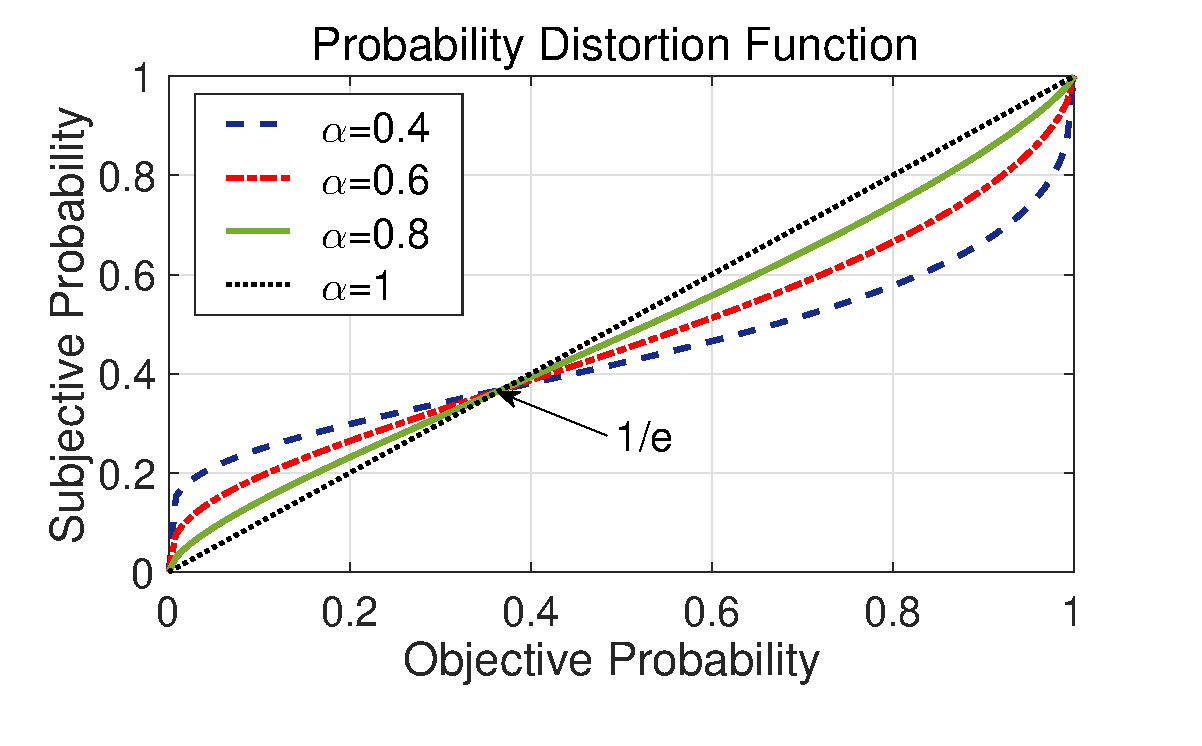
\includegraphics[scale=0.58]{./pic/dist_func.eps}
%\caption{Probability distortion functions under different distortion parameters $\alpha$.}\label{fg:dist_func}
\caption{失真参数$\alpha$不同取值下的概率失真函数。}\label{fg:dist_func}
\vspace{0.1cm}
\centering
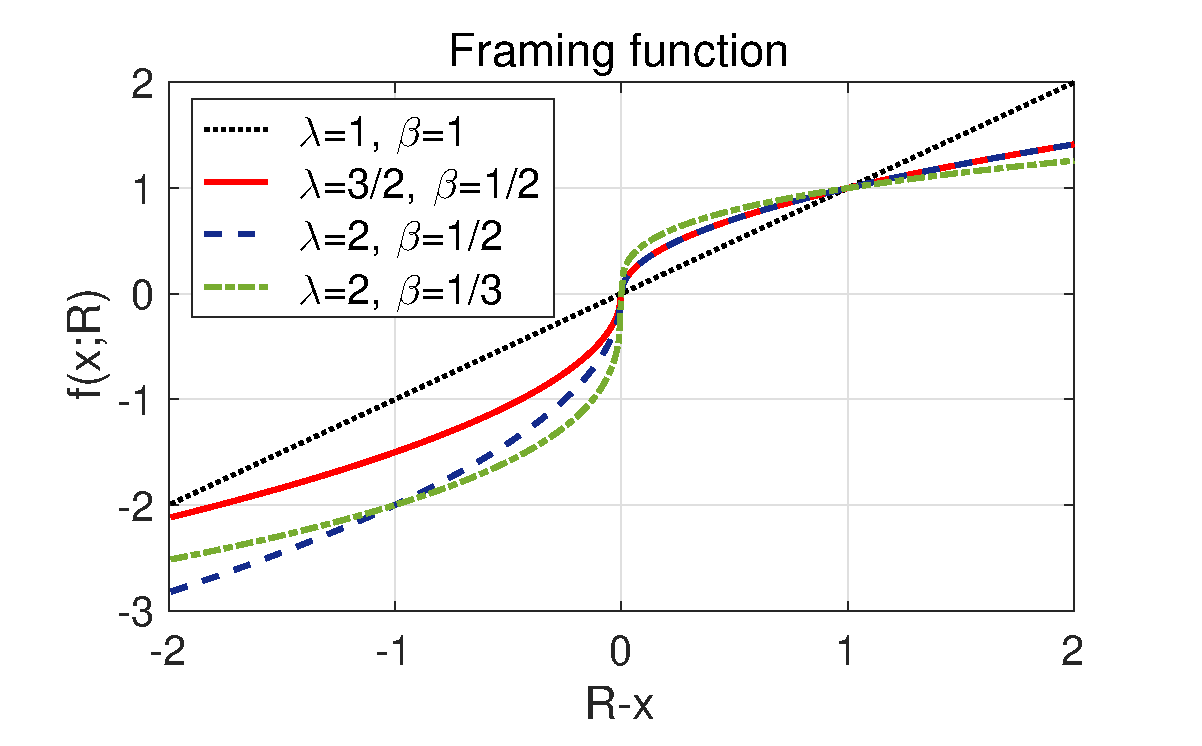
\includegraphics[scale=0.58]{./pic/fram_func.eps}
%\caption{Framing functions under different utility aversion parameters $\beta$ and loss penalty parameter $\lambda$.}\label{fg:fram_func}
\caption{不同效用规避参数$\beta$和损失惩罚参数$\lambda$下的框架函数。}\label{fg:fram_func}
\end{figure}

我们考虑的前景理论的另一个特征是\emph{效用框架效应}。此效应反映了每个服务提供商对自己的收益进行主观评估的实际情况。实际中,仅当其收入超过参照点$R$($R$无需等于零)时,每名用户才会将其视为收益增益,否则将视为收益损失。同样,在给定参考点$R$的情况下,S型单调框架函数$f(\cdot)$会进一步调整客观收入,其中函数在$v>R$侧为凹函数,而在$v<R$一侧是凸函数。此外,在$R$附近,收益损失比收益增益增长得更快,表明收益损失的边际效用大于收益增益的边际效用。常用的框架函数为Kahneman框架涵是\cite{Kahneman},
%Another characteristic of Prospect Theory we considered is the \emph{utility framing effect}. This effect captures the practical situation where each service provider has subjective evaluation of her own payoff. In practice, each user might consider her payoff as a gain only if it is above a reference point $R$ (not necessarily equals zero), and consider it as a loss otherwise. Also, given the reference point $R$, the objective payoff is further tuned by a S-shaped monotone framing function $f(\cdot)$, which is concave at the side where $v>R$, and convex at the side where $v<R$. In addition, in the neighborhood of $R$, the losses loom larger than gains indicating that the marginal utility in losses is larger than in gains. In this work, we use a framing function based on the one proposed in \cite{Kahneman},
\begin{equation}\label{eq:framing}
f(x;R)=
\begin{cases}
(v - R)^{\beta}, &v\geq R\\
-\lambda(R-v)^{\beta}, &v<R
\end{cases}
\end{equation}
其中参数$0<\beta\leq 1$和$\lambda\geq 1$分别用于刻画风险规避和损失规避的因素。图\ref{fg:fram_func}展示了不同参数取值下的框架函数。特别地,当博弈参与者收入远离参照点时,$\beta$值越大,表示风险规避程度较小;$\lambda$值的增大则刻画了博弈参与者在客观上经历等同的收益的损失和增益时,所主观上体验到的损失要大于所体验到的增益。容易看出,当$\beta=\lambda=1$时,主观收益曲线与原始的客观收益曲线一致。
%我们假设每个服务提供商$k$基于式(\ref{eq:framing})来评估其收入。则在前景理论模型下,服务提供商$ k\in\K$的预期收入$z_k^{PT}$可写为
%where the parameters $0<\beta\leq 1$ and $\lambda\geq 1$ model the risk aversion and loss aversion respectively. Fig. \ref{fg:fram_func} illustrates the framing function with different parameters. In particular, a larger $\beta$ characterizes less degree of risk aversion when the player's payoff is away from the reference point; and a larger $\lambda$ captures the greater loss experienced by the player with her payoff being reduced by a certain amount, in comparison to the corresponding gain she experiences with the same amount of the payoff increase. It is easy to see that when $\beta=\lambda=1$, the subjective payoff boil down to the original objective payoff. We assume each service provider $k$ evaluate her revenue using (\ref{eq:framing}) with parameter $\beta_k$, and reference point $R_k, \forall k\in\K$. Under Prospect Theory model, the expected revenue $z_k^{PT}$ of service provider $k\in\K$ can be written as

%\begin{equation}\label{eq:PT}
%%\small
%z_{k}^{PT}(\pi_{k},\pi_{-k})=\sum_{\mathbf{p}\in \mathcal{P}}\pi_k(p_k)w\left(\prod_{k'\in\K,k'\neq k}\pi_{k'}(p_{k'})\right)f_k(v_k).
%\end{equation}
%
%我们将前景理论讨论下的定价博弈表示为$\mathcal{G}_P^{PT}\left(\mathcal{K},\Delta\mathcal{P},\{z_k^{PT}(R_k)\}_{k\in\mathcal{K}}\right)$,然后在下一节中重新讨论价格博弈的均衡解的存在。
%We denote the pricing game under Prospect Theory as $\mathcal{G}_P^{PT}\left(\mathcal{K},\Delta\mathcal{P},\{z_k^{PT}(R_k)\}_{k\in\mathcal{K}}\right)$, and revisit the existence of equilibrium solution for the pricing game in the next section.



\section{本章小结}\label{chp2:sec:con}
